\documentclass[11pt]{article}
\usepackage{graphicx}
\usepackage{amsmath,amssymb, amsthm}
\usepackage{color}
%\usepackage[hidelinks]{hyperref}
\usepackage{hyperref}
 \usepackage{amsfonts}
 \usepackage{makeidx}
 \usepackage{xfrac}
 % \usepackage{ulem}
 \usepackage{tikz}
 \usetikzlibrary{arrows}
 \usepackage{natbib}
 %\bibliographystyle{chicagoa}
 \makeindex
      
\textwidth = 6.5 in \textheight = 8.5 in \oddsidemargin = 0.0 in
\evensidemargin = 0.0 in \topmargin = 0.0 in \headheight = 0.2 in
\headsep = 0.5 in
\parskip = 0.2in
\parindent = 0.2in

\newcommand{\cyp}{\citeyearpar}
\newcommand{\ha}{\frac{1}{2}}
\newcommand{\R}{\mathbb{R}}
\newcommand{\C}{\mathbb{C}}
\newcommand{\CP}{\mathbb{CP}}
\newcommand{\PP}{\mathbb{P}}
\newcommand{\N}{\mathbb{N}}
\newcommand{\Q}{\mathbb{Q}}
\newcommand{\Z}{\mathbb{Z}}
\newcommand{\B}{\mathbb{B}}
\newcommand{\A}{\mathbb{A}}
\newcommand{\Hom}{\rm{Hom}}
\newcommand{\F}{\mathbb{F}}
\newcommand{\ii}{\sqrt{-1}}
\newcommand{\ph}{\varphi}
\newcommand{\rd}{\partial}
\newcommand{\dux}{\frac{\partial u}{\partial x}}
\newcommand{\duy}{\frac{\partial u}{\partial y}}
\newcommand{\dvx}{\frac{\partial v}{\partial x}}
\newcommand{\dvy}{\frac{\partial v}{\partial y}}
\newcommand{\ulr}{\underline{r}}
\newcommand{\ulu}{\underline{u}}
\newcommand{\ulv}{\underline{v}}
\newcommand{\ulg}{\underline{g}}
\newcommand{\ulga}{\underline{\gamma}}
\newcommand{\olb}{\overline{\B}}
\newcommand{\dsp}{\displaystyle}
\newcommand{\gdg}{\emph{Grundlagen der Geometrie}}
\newcommand{\n }{^{-1}}
\newcommand{\rr}{\mathbf{r}}
\newcommand{\col}{\textcolor}
\newcommand{\ci}{\mathcal{I}}
\newcommand{\cz}{\mathcal{Z}}
\newlength{\wdth}
\newcommand{\strike}[1]{\settowidth{\wdth}{#1}\rlap{\rule[.5ex]{\wdth}{.4pt}}#1}


\newcommand{\mm}{$\mathbf{m}$}
\newcommand{\rrt}{Riemann--Roch Theorem}
\newcommand{\dieq}{dialytic equation}
\newcommand{\chnr}{characteristic number}
\newcommand{\moeq}{modular equation}
\newcommand{\nft}{Noether's Fundamental Theorem}
\newcommand{\cbt}{Cayley--Bacharach theorem}

\def\PP{{\mathbb P}}

\newtheorem{theorem}{Theorem}
\newtheorem{lemma}{Lemma}
\newtheorem{corollary}[theorem]{Corollary}
\newtheorem{definition}{Definition}
\newtheorem{example}{Example}
\raggedbottom

\def\de#1{{{\bf \col{red}{David says [* }\col{red}{#1{\bf\ *]} }}}}
\def\jg#1{{{\bf \col{red}{Jeremy says [* }\col{red}{#1{\bf\ *]} }}}}



\begin{document}

\section{A historical essay on some topics in algebraic geometry}
This essay offers a brief overview of aspects of the long history of plane curves and algebraic geometry.\footnote{I am grateful to Andrea del Centina for letting me read the manuscript of his forthcoming book \emph{The History of Projective Geometry}, which has been very helpful and will surely become the definitive work on the subject.}   

\subsection{Greek mathematicians and conic sections}
The first mathematicians to have studied curves more complicated than the straight line and the circle seem to have been those of ancient Greece.  Surviving sources suggest that the study of conic sections, literally sections of a cone, may well have arisen with Menaechmus's work on doubling the cube around 350 BCE. This was a long-standing problem that was given a theological spin in the form of the Delian problem, which, according to one story, asked for an altar double the size of a given one, apparently to get rid of a plague. Finding this difficult, workers consulted Plato, who said that the real reason for the task was to reproach the Greeks for their neglect of geometry.\footnote{Theon of Smyrna, 2nd century CE, in (Thomas 1939, Vol. 1, 257).}
It may well also have stood out because Plato in the \emph{Meno} dialogue made such a fuss of doubling the square. Hippocrates of Chios, who flourished around 470 BCE,  had already reduced the problem to that of finding two mean proportionals between 1 and 2; i.e. the numbers $x$ and $y$ such that 
\begin{equation}~\label{Menmus}
1:x= x:y = y: 2.
\end{equation}
For Greek mathematicians, these would have been line segments of those lengths. Many solutions to the problem of finding two mean proportionals were proposed; Menaechmus, a younger associate of Plato and a pupil of Eudoxus, may have been the first to connect the problem of doubling the cube to the idea of conic sections, or perhaps we should say quadratic curves, because it has been argued that he considered equation \eqref{Menmus} as defining or generating curves that would have been drawn and understood pointwise. At all events, he expressed the solution to the Delian problem in terms of the intersection of a hyperbola and a parabola.\footnote{See Eutocius \emph{Commentary on Archimedes' Sphere and Cylinder}, in (Cohen and Drabkin 1948, 62--66). Among Eudoxus's many achievements is to have provided the first theory of magnitudes that went beyond the rational numbers; it is now found in Book V of Euclid's \emph{Elements}.}

About a century after Menaechmus, Diocles, and soon after him Apollonius, made significant progress with the conic sections, and the transformation from what Menaechmus did in solving problems to identifying a family of curves may be due to one Aristaeus, whose work is now lost. Diocles identified the curve that would focus the sun's rays to a point as the parabola, and knew precisely how to cut a cone so as to obtain it. 

Apollonius produced the first \emph{theory} of conic sections as sections of a cone. The books are very dry. Van der Waerden called him a virtuoso ``in dealing with geometric algebra, and also a virtuoso in hiding his original line of thought'', while going on to say that ``his reasoning was crystal clear and elegant.''\footnote{See (Van der Waerden 1961, 248).} It's hard to summarise Apollonius's work. He began with basic definitions of a cone (on a circle) and its three types of section: the hyperbola, parabola, and ellipse; the names are due to him. He showed that all the known sections that had been studied as sections of a cone with vertical angle a right angle could be obtained as sections of a suitable but otherwise arbitrary cone.\footnote{In many ways, the first place to go for an account of Greek mathematics remains Sir T.L. Heath's century-old account (Heath 1921), but it should be supplemented by more modern readings, such as (Knorr  1993).}

It's entirely arguable that a system of coordinates was present in his work, inasmuch as he generally referred everything to a pair of distinguished lines in the plane of section of the cone, but it is buried in the heavy use of proportion theory between different line segments, and you have to be very smart, as Apollonius undoubtedly was, to handle it. That said, he produced a theory of the principal diameters of conics, studied such problems as finding the tangents to a conic from an exterior point, and came close to observing the properties of cross-ratio that modern writers were to detect. He also had a theory about normals to conics from which  it's a short step to obtaining their evolutes. The biggest weakness in Apollonius's theory was that very often he had to treat the three kinds of conic section separately, although you can see him trying for greater generality. 

We know Apollonius's theory of conic sections because we are fortunate that  four books of his conics survive in Greek and three more in Arabic; the eighth and final volume is lost. He also studied several particular problems, the solution to which required knowing properties of conic sections.  However, although a number of other Greek mathematicians pitched in, little of  their work survives directly, more does in the work of later writers such as Pappus; and much of it, including a book by Euclid, who lived a little before Apollonius, is lost. 

A small number of other curves were studied by Greek mathematicians, of which probably the one best known today is the spiral of Archimedes (which has polar equation $r = a \theta$) and was introduced for the purpose of squaring the circle. A curve introduced by Diocles for the purpose of finding two mean proportionals between $a$ and $b$ can be given the Cartesian equation $y^2 (a + x) = (a-x)^3.$ For a fuller account, see (Heath 1921, Vol. 1, Ch VII). 

Mathematicians of the Islamic era also studied conic sections and the various problems they inherited from the Greeks. For example, Omar Khayy\={a}m gave a complete account of how to solve cubic equations using pairs of conic sections where necessary.\footnote{See (Khayy\={a}m 1950).}

At this point, the history of algebraic geometry broadly divides into two. One part concerns the theory of conic sections -- algebraically, curves of degree two -- and the other the theory of curves of higher degree. The first can regard Girard Desargues as a major innovator, the second his contemporary,  Ren\'e Descartes. Let us take the study of conic sections first, and trace how it leads to the concept of a projective space.


\subsection{Conic sections from the 17th to the 19th centuries}
In 1639 Desargues published fifty copies of a short pamphlet entitled \emph{Brouillon Project d'une atteinte aux evenements des rencontres du cone avec un plane} (\emph{The Rough Draft for an Essay on the results of taking plane sections of a cone}) (1639), on what we could call the projective theory of conics.\footnote{English translation in (Field and Gray 1987).} He was perhaps hoping for useful critical feedback, but he never returned to rewrite his account.  In the essay, all non-degenerate conics are treated on a par, and treated as perspective images of the circle. The idea that all (non-degenerate) conics are the projective image of a circle is not original with Desargues. It was stated by Maurolico, for example, in his book \emph{Theoremata de lumine et umbra} (1611), which it is likely Desargues knew, and in any case it is visually apparent to anyone who thinks of the conics as sections of a cone on a circular base. The trick is to make this insight work.

Desargues's key idea is that of properties of figures invariant under projection, such as the cross-ratio of four points on a line: if $A,  B, C, D$ are four points on a line, their cross-ratio can be defined to be
$\dfrac{AC.DB}{AD.CB}$. The special case,  when the cross-ratio is $-1$ and $AC/CB=-AD/DB$ and people said $B$ and $D$ separate $A$ and $C$ in the same ratio, arises frequently in the theory of the poles and polars of conic section. Desargues also had a more complicated property of six points, which, like the four-point property, was invariant under a projection. He connected all this to the study of the ``complete quadrilateral'' -- take four points, no three collinear, and join them in all possible ways --  and thence to the study of conics through those four points. 

\bigskip
\begin{center}
    \begin{figure}
   \begin{center}  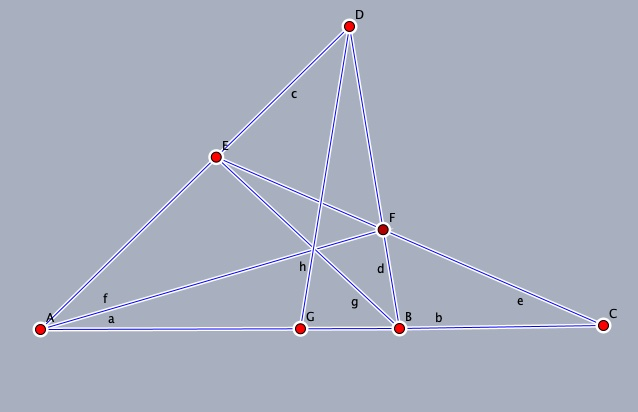
\includegraphics[width=30em]{CompleteQuad3.png} 
   \end{center}
     \protect \caption{A complete quadrilateral}
      \label{figCompleteQuad}
     \end{figure}
\end{center}

\bigskip 





The  \emph{Brouillon Project} is fiercely unreadable.\footnote{Happily, it has been the subject of sequence of detailed analyses in recent papers by Marie  Anglade and Jean-Yves Briend; see (Anglade and Briend 2022) and the references to their earlier papers cited there.} It was also lost for a long time and known only through commentaries by later authors until Michel Chasles found a handwritten copy made by Philippe de la Hire in 1845.\footnote{The only known copy of the original \emph{Brouillon project} turned up in 1950.} In particular, de la Hire, a generation after Desargues, wrote some much more readable, and longer, works in Desargues's spirit, illuminating the role of cross-ratio in the theory of tangents that came close to a theory of duality. Desargues's famous theorem on two triangles in perspective was published separately in (Bosse 1648).

The best attention Desargues's little book got was from his younger contemporary Blaise Pascal, who evidently produced a virtually complete theory of conics around what he called the ``mystical hexagram''. Unhappily much of it is lost, and known to us only from some notes on it made by Leibniz, but the idea is that while there is always a conic through five points something happens if you want a conic through six points: we call it Pascal's theorem. Then, if you let the sixth point collapse onto one of the other five you get a tangent to the conic through those five points. One way or another all the key properties of conics are wrapped up in this idea, or so Pascal seems to have shown, and much of the early 19th century work in France can be seen as attempts to recover such a theory. It includes such topics as duality, in the form of the pole and polar relationship with respect to a conic, more or less known earlier to de la Hire.\footnote{For a thorough analysis of Pascal's work and its context, see (Del Centina 2020).} 


Thereafter, truly projective geometry languished for much of the 18th century, despite some insightful contributions by Newton that we shall mention below (see p. ~\pageref{Newtonconics}). Its revival is conventionally dated from the early work of Gaspard Monge, who as a young man seeking a job in the French army was  interested in how to depict three dimensions on two. He devised a method of plan and elevation (projections onto a horizontal and a vertical plane) that he could couple to some simple algebra in a way that was easy to use; he was offered a job at the military Academy in M\'ezi\`eres and his discovery made a military secret. During the French Revolution, Monge was influential in setting up the Ecole Polytechnique, where he was an inspiring teacher of geometry, and this did much to revive the subject. 

Among those so inspired there was Jean Victor Poncelet, who promoted a much more general theory of transformations with a view to unifying the theory of conics that he began to develop while a prisoner-of-war in Saratov during Napoleon's disastrous invasions of Russia. His \emph{Trait\'e des Propri\'et\'es Projectives des Figures} (1822) is a visionary textbook that relies on some rather mysterious arguments about ideal points of intersection (Cauchy, who reviewed the book, urged that they be regarded as points with complex coordinates; Poncelet never agreed). As a result, some of the transformations it invokes necessarily require complex coordinates. The most famous result in the book is Poncelet's closure theorem, which has continued to attract attention to this day, but it is also notable for many other theorems involving pairs of conics.\footnote{For an interesting  set of essays analysing what projective space might be and how it came about, including an extensive analysis by J.-P. Friedelmeyer of the work of Poncelet, see (L. Biosemat-Martagon 2010).}

In the 1820s, Poncelet had a dispute with Joseph Diaz Gergonne, the editor of the only journal at the time entirely devoted to mathematics, about what duality in the plane actually is. Poncelet always saw it as pole and polar with respect to a conic, Gergonne saw it as a new and fundamental feature of projective geometry.\footnote{See (Gergonne 1826).} This led into confusion when applying it to curves of degree three of more, a matter that began to be sorted only with Pl\"ucker's work, as we shall see below.


Another mathematician who was inspired by Monge was the Frenchman Michel Chasles, who used the projective invariance of the cross-ratio of four points to eliminate much of the weirdness of Poncelet's ideas. Independently, Jakob Steiner did very similar work in Germany. He can be credited with the first truly projective definition of a conic section. Even so, there remained an irritating feature of cross-ratio: it was given as a function of four lengths, but length is a property of Euclidean geometry, not projective geometry.  If projective geometry is to be regarded as more fundamental than Euclidean geometry, because it rests on fewer assumptions or axioms, then the intrusion of Euclidean length in the definition of cross-ratio is at the very least unfortunate. Nor can one easily speak of there being a concept of projective space in the 1820s; rather, much of geometry at this time was about figures in the plane subject to a variety of projective transformations. The first truly foundational work on real and complex projective geometry that avoided deriving it from Euclidean geometry was the achievement of von Staudt in his \emph{Geometrie der Lage} (1847), in a long and difficult work that influenced Felix Klein when he succeeded von Staudt as a Professor at Erlangen a few years later. 

All in all, a surprising amount of work was done on the theory of conic sections  at the start of the 19th century, and before it is dismissed as arcane it should be stressed that the subject was a proving ground for the development of projective geometry. Two approaches stand out: the search for entirely  general methods that would treat all non-degenerate conics on a par; and the emergence of the property of duality. Matters are complicated by the existence of two separate traditions, usually called the synthetic and the analytic, supposedly divided into classical geometric methods and more algebraic ones that introduce coordinates. 
Recent historical work suggests that it was all a bit murky, and algebraic methods were also often used in synthetic geometry. Several things promoted the use of synthetic methods. They can be elegant when algebraic methods are blunt; they correspond to the visual form of the conics; they provide a language for describing what is apparent or to be found in a problem. Against them is the obstinate fact that algebra is more general: it does not care if some quantities become negative, but what is a negative length? Once ways round that were found (by Poncelet and then Chasles) the way was open to a truly systematic synthetic theory of conics.   

How then did this change, and purely synthetic projective geometry begin to wane? Very few of the original protagonists disdained algebra outright, and as the (projective) theory of conics reached completion in the 1820s and established its fundamental character, being more general than metrical Euclidean geometry, it also had its baroque aspects. But worse, it did not generalise at all readily  to the study of curves of higher degree. For that, as even Newton had recognised, a hefty dose of algebra was required.







\subsection{Descartes,  coordinatising the plane,  graphing  curves}
A common way to think of curves in antiquity was pointwise: some length depends in a given way on some other length. Accordingly, at least in principle, if you know the independent length
(the ordinate, or $x$ coordinate) you know the dependent length (the abscissa, or $y$ coordinate).  

By Descartes' time there was already some sophisticated algebra expressed in a formalism that hadn't quite shaken off   the Greek insistence on seeing everything as geometrical magnitudes: lengths, areas, volumes, and, well, what exactly? The French mathematician Fran\c{c}ois Vi\`ete in his \emph{Isagoge} boldly spoke of magnitudes having the dimensions of side, square, cube, square-square, square-cube and so on.\footnote{See his collected works, (Vi\'ete 1646).} It was possible to write polynomial equations in this language, as Vi\`ete did in the early 1600s. First Fermat in 1636, and then much more boldly Descartes in 1637, realised that you could extend the language to two variables and so describe curves in the plane.



\bigskip
\begin{center}
    \begin{figure}
   \begin{center}  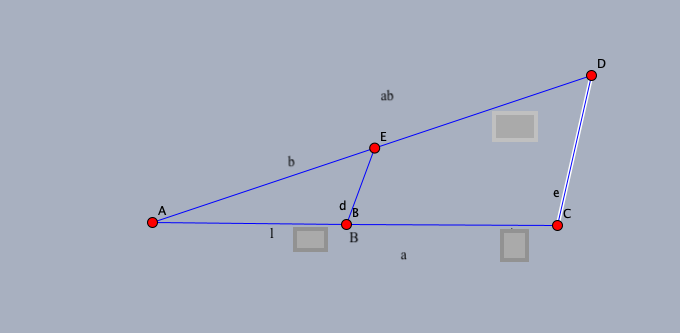
\includegraphics[width=30em]{Multiplication.png} 
   \end{center}
     \protect \caption{If $A$ is of length 1, $AC$ of length $a$, $AE$ of length $b$, and $BE$ and $CE$ are parallel then AD is of length $ab.$}
      \label{figMacaulay}
     \end{figure}
\end{center}

\bigskip 

Descartes's first achievement in his \emph{La G\'eom\'etrie} (1637) was to eliminate the dimensional aspect. A simple use of similar triangles allowed him to show that the product of two lengths could be seen as another length (not an area) so all geometrical quantities could be regarded as one-dimensional and the idea of dimension quietly dropped. Then came the real work. Almost all mathematical problems in his day were expressed in the language of geometry, except for some problems we would call diophantine and were implicitly about integers and rational numbers. Accordingly, the answer had to be expressed geometrically. Descartes's idea was to give letters to all the lengths involved in a problem, use the statement of the problem to express relationships between the letters, and reduce the equations to a single equation. Then solve the equation and express the answer again in geometrical terms.  

His achievements include replacing Vi\`ete's cumbersome algebra, which was written in capital letters with verbal abbreviations for the algebraic operations, with something much more like   what we use today.  He wrote $x$ and $y$ for the key variables (not $A$ and $E$ in the manner of Vi\`ete). Descartes was clear that he was using coordinates, although his $x$ and $y$ coordinates could have oblique axes. In this way he solved the famous Pappus problem: given four lines and four angles (nothing is lost if take these angles to be right angles), find the locus of points $P$ such that the product of the distances of $P$ from the first two lines is proportional to the product of the distances of $P$ from the last two lines. As he showed, and Pappus had known, the answer is a conic section, but  Descartes went further and claimed that in this way he could solve the Pappus problem for any number of lines. 

This was to infuriate Newton, who showed that Greek methods were indeed adequate to the original Pappus problem. The background here is that Newton was also engaged in demolishing Descartes's theory of planetary motion in favour of his own, which led him into the theory of conic sections and to pose and solve problem of finding the conic (or conics) through $n$ points and tangent to $5-n$ lines, which he did in Book I, Section 5 of his \emph{Principia Mathematica}.~\label{Newtonconics}

It can be argued that the theory of specifically algebraic curves has its origin in Descartes's method for finding normals to a curve at a point, which  involved considering all the circles through the given point and imposing the condition that the equation for the circle be such that it passes twice through the given point. On the basis of three examples, he claimed that the method always worked  if the curve had an algebraic equation; curves like the cycloid that were patently not algebraic he sought to exclude from geometry, something else that annoyed Newton. and described a system of linkages (sliding rulers) that he said could be adapted to draw any such curve.

In the 1660s and 1670s, but only published  the 1690s and again in 1704 as an Appendix to his \emph{Opticks} Newton worked on a classification of cubic curves. He claimed that there were 72 distinct types which could be derived by simplifying the general equation using what we would call affine or linear transformations, although at one point he used a simple birational transformation. For some reason, in writing up his work for publication he omitted four of the possible cubics, and they were speedily found by various other mathematicians.  Newton also made the striking remark that this collapses to five types if projective transformations are allowed. 





A plane cubic curve is defined by an equation involving ten coefficients, or more precisely by the nine ratios between the coefficients, which suggests that it should be determined by nine points in the plane because their coordinates provide nine equations that should determine these nine ratios.  The Scottish mathematician Colin MacLaurin not only knew this, but knew in 1720 that there were problems with it: any two cubics will meet in nine points, and so these nine points do not determine a unique cubic, and indeed there will be infinitely many cubics through these nine points.\footnote{MacLaurin also knew that a general cubic curve has nine flexes, and the line joining any two passes through a third.}  MacLaurin did not, however, know how to solve this puzzle. His observation was conveyed to Euler by his friend the Swiss mathematician Gabriel Cramer  in 1744. This apparent contradiction with the claim that nine points in the plane always determine a unique cubic is today known as Cramer's paradox. When Cramer addressed the problem in his book (1750, Chapter 3) he suggested that nine points determine a cubic unless they are nine points common to two cubics, but he offered no proof of this result. He did, however, also suggest that if the $\ha (n+1)(n+2)$ points needed the determine a curve of degree $n$ contain $tn$ common to a curve of degree $t < n$ then the curve through the  $\ha (n+1)(n+2)$ points breaks up into two curves, one of which passes through the $tn$ points.


The claim about cubic curves , and more generally the analogous claim for curves of degree $n$, which are determined by $\ha n(n+3)$ general points, was repeated  by  Euler  in the second volume of his \emph{Introductio} (1748). He then wrote a paper (Euler 1750) in which he attempted to resolve the paradox, but  he did not get very far.  He began by supposing  that eight points in the plane are given that impose eight independent conditions on the cubic. If these eight points are eight points common to the given cubic and another, then the ninth point common to those cubics cannot impose a new condition on the coefficients, and so, he said, the ninth equation might be identical with one of the previous eight. 
Euler\index{Euler, Leonhard (1797--1783)} lived any theory of linear dependence was available, so he did not claim instead that the equation it imposes on the coefficients must be a consequence of the first eight equations. He did however solve the problem explicitly for those cases when five points do not determine a conic, which happens when four lie on a line.



The idea that algebraic curves of degrees $k$ and $m$ in the plane should meet in $km$ points was something of a folklore result in the early 18th century, but it travelled without a proof or many years. Euler discussed it in the second volume of his \emph{Introductio in Analysin Infinitorum} (1748) and noted that even in simple cases  for the counting to work one would have to take care of multiple points (such as tangents),  points `at infinity' (consider a parabola and a line parallel to its axis), and allow the  coordinates of intersection points to be complex (consider the intersection of two circles). The first person to find a persuasive way of tackling the problem was \'Etienne B\'ezout, who lived from 1739 to 1783, and made his living teaching mathematics at the French military and naval academies. He published the theorem that bears his name in a book of 1779; it is based on his theory of the resultant of two polynomial equations that he developed in a paper of 1764. His proof of the theorem is gappy and intuitive by any standards, but so much better than what had been done before that his immediate successors were willing to give him real credit for doing as much as he did. His results inspired later work by Cauchy and Sylvester.

All things considered, progress in the study of cubic, quartic, and higher degree curves in the 18th century was piecemeal and slight, and the sheer enormity of the equations involved seems to have baffled even Euler. New methods for handling such curves would have to be found, such as came in with Julius Pl\"ucker in the 1820s. His key idea was to study families of curves, using the symbolic notation devised by Gergonne.\footnote{See  (Gergonne 1826--1827), (Pl\"ucker 1835) and (Pl\"ucker 1839).} If $S_1$ and $S_2$ stand for the equations of two curves of the same degree, then $S_1 + \lambda S_2$ is the equation of another degree of that kind. This allowed him to pull out geometrical properties of cubic and quartic plane curves while avoiding the algebraic complexities that had defeated Euler.  

Pl\"ucker also resolved the paradox in the theory of plane curves in his (1834) that had stumped Gergonne and Poncelet, by making a more insightful use of the role played by the singular points on a curve than Poncelet had done. By duality, the degree of the dual to a given plane curve $C$ is the number of tangents that can be drawn to the curve through an external point. If we work affinely, we can write the equation of the curve as $f(x, y) =0$ and the equation of a line through the given point in the form $y = ax + b.$ Points where this line meets the curve are the solutions of the equation $f(x, ax+b)=0$, and points where this line meets the curve twice or more are those where the equation $f(x, ax+b)=0$ has a repeated root. In general, when $f$ is of degree $n$ this is a condition of degree $n-1$, and so there are $n(n-1)$ tangents to the curve $C$ through an external point. Therefore, the degree of the dual curve to a curve of degree $n$ is $n(n-1).$

The paradox arises because the dual of the dual curve ought to be the original curve, but the dual of the dual apparently has degree $n(n-1)(n(n-1)-1).$ When, for example, $n=3$, $n(n-1) = 6$ and $n(n-1)(n(n-1)-1) = 30.$ Plainly, this does not return the original curve. Pl\"ucker's response, which would strike us today as at best heuristic, was that any line through a double point, say, is counted in this way as a tangent, and this throws the count of genuine tangents off. More precisely, he  showed that each node on a curve reduces the degree of the dual curve by 2, and each cusp reduces it by 3. Consequently, he claimed that  a curve of degree $d$ with $\delta$ double points and $\rho$ cusps has a dual curve  of degree $d(d-1) -  2\delta - 3\rho.$ 


Pl\"ucker also showed in his (1839, 207--227) that the nodes of $C^{*}$  corresponded to the bitangents of $C$, while the cusps of $C^{*}$ corresponded to the flexes of $C$, and vice versa. To see how he resolved the duality paradox, consider  the case of a non-singular cubic curve. It has no nodes, cusps, or bitangents, and as yet an indeterminate number, $j$ of flexes. Its dual has degree 6 and $j$ cusps. The dual of the dual curve therefore has degree $6.5 - 3j$, which will equal 3 if $j = 9.$ As we saw, the result that a non-degenerate cubic curve has nine flexes had been known since MacLaurin. For curves of higher degree, it is necessary to consider a curve of degree $n$ that has $\delta$ double points, $\kappa$ cusps, $\tau$ bitangents, and $\iota$ inflections. Suppose that its dual has degree $n'$. Pl\"ucker argued that
\[n = m(m-1) - 2\delta - 3 \kappa,\]
\[{\rm and}\; \iota = 3m(m-2) - 6\delta - 8\kappa,\]
with another formula for $\tau$, along with the corresponding formula for the dual curve and its inflection points and bitangents.

The number $\iota$ is most easily found using an argument due to Hesse, who showed  in his (1844),  that the set of flexes $\Gamma\subset G$ on a curve $G$ of degree $d$ with equation $F(x, y, z) = 0$ could be characterized as the intersection of $G$  with the curve $D$ defined by the vanishing of the \emph{Hessian determinant}:
$$
H = \det \begin{pmatrix}
 \partial^{2}F/\partial x^{2} &\partial^{2}F/\partial x\partial y &\partial^{2}F/\partial x\partial z \\
\partial^{2}F/\partial x\partial y  &\partial^{2}F/\partial y^{2} &\partial^{2}F/\partial y\partial z \\
\partial^{2}F/\partial x\partial z &\partial^{2}F/\partial y\partial z &\partial^{2}F/\partial z^{2} 
\end{pmatrix}.
$$
Since the entries of this matrix have degree $n-2$, the degree of $H$ is $3(n-2).$ For general $F$ the curves $G$ and $D$ meet transversely, so B\'ezout's Theorem shows that a general curve of degree $m$ has exactly $\iota = 3n(n-2)$ flexes.\footnote{This result was first proved in a different way in (Pl\"ucker 1835, 264), as Hesse acknowledged.}

The most famous case Pl\"ucker established in  his book (1839, 247),  concerns   a nonsingular plane curve $C$ of degree $n=4$  (no nodes, cusps, or other singular points) having $\tau$ bitangents and $\iota$ flexes.   Its dual curve has degree 12 and will have $\tau$ double points and $\iota$ cusps, and the dual of the dual will have degree 
$12\cdot 11 - 2\tau - 3h  = 4.$ 
Hesse's theorem shows that $h = 24$ (Pl\"ucker\index{Pl\"ucker, Julius (1801--1868)} had an ad hoc argument to the same effect)  and so $b = 28$,  and we  see that $C$ has exactly 28 bitangents. Pl\"ucker showed that they can all be real.

In 1849, Pl\"ucker gave up mathematics for physics, particularly the study of cathode rays; he was awarded the Royal Society of London's Copley medal (its highest honour) for this work in 1866. He had by then returned to the study of geometry in 1864, but now in the field of line geometry, which he transformed into a new branch of geometry. 

\bigskip

\begin{center}
    \begin{figure}
   \begin{center}  \includegraphics[width=15em]{28bitangents} 
   \end{center}
     \protect \caption{\, Pl\"ucker's quartic curve has 28 bitangents, from (Pl\"ucker 1839)}
      \label{fig28bitangents}
     \end{figure}
\end{center}
\bigskip

Pl\"ucker's formulae work well for curves of degrees 3, 4, and 5, but not so well thereafter.  He listed all the solutions he could find to the equations that bear his name up to curves of degree 10, but he did not discuss the kinds of singularities a curve may have that are not of the type he had considered.\footnote{See (Pl\"ucker 1839, 214).}  Progress was only made with a paper by Cayley (1866), who drew on Puiseux's paper (1850) that analysed  of how curves are ramified at a singular point,  showed how the branches are permuted in cycles, and how this is captured by the local power series expansions, which begin with fractional indices.\footnote{Cayley's paper was corrected by Otto Stolz in his (1875), who found that the conclusions were correct but the proof ``as he [Cayley] himself remarks'', was not quite complete.}

Puiseux was one of a number of mathematicians in the circle around Cauchy. Cauchy had spent the 1830s and early 1840s following the Bourbon Court around Europe from a strange belief that the oath of allegiance he had sworn to the crown on becoming a professor compelled him to do so. As a result, by 1850 few people knew the work he had done in those years, and even he seems to have forgotten what he had done in complex variable theory back in the 1820s, which included a version of what we call the Cauchy integral theorem restricted to rectangular contours. Only on his return to Paris did he begin to think much more geometrically; previously his attitude to a many-valued `function' was to cut the plane and study just a branch of it on what remains. His understanding of branch points was quite limited, and this left space for Puiseux to study integrals on arbitrary contours   and what happens to integrals taken around branch points. 

\subsection{The birth of projective space}
When did projective space come in, regarded as something more rigorous than Euclidean space with a ``line at infinity''? This might simply be a suitable set of coordinates. Pl\"ucker used coordinates for the plane with a line at infinity in his (1830) with a view to enabling homogeneous equations to correspond to curves; in this system the coordinates $(p, q, r)$ denote the signed distances of a point from the three sides of a triangle of reference.\footnote{These are not projective coordinates because any one of $p, q, r$ is a function of the others.} However, in his study of curves (1835) he would first discuss them in  the plane, and then as they went off to infinity; he didn't say that the line at infinity could be mapped by a projective transformation into the finite part of the plane.  The way forward was indicated by M\"obius, who introduced barycentric coordinates in his (1827). Pick three points forming a triangle, say $ABC$, and attach weights, positive, zero, or negative (not all zero) to these points. The barycentre or centre of gravity of these three weighted points is a point $P$ which can be said to have those three weights (or, better, their ratios) as its barycentric coordinates. If you put the points $A, B, C$ at, say,  $(0, 0), (1, 0), (0, 1)$ you get an easy way to relate points in what could be called the Cartesian and barycentric coordinate planes. The big plus is that the line at infinity, which is invisible in Cartesian coordinates, is a perfectly sensible line in barycentric coordinates. In this way M\"obius obtained a simple theory of conics and duality in the plane. (He also showed that there are dualities in $P^3$ that are not pole-polar dualities.)

If you drop the talk about weights, and keep the idea that barycentric coordinates are best thought of as ratios of three numbers, you have projective coordinates; this was one of the contributions of Otto Hesse in the 1840s.\footnote{See, for example, his (1844).}
Mathematicians were still reluctant, however, to decide if this space was $\R P^2$ or, less likely, $\C P^2$.
 
Throughout the 18th century mathematicians had become more and more comfortable with the idea of complex numbers in algebra, and with the idea of proving that a polynomial of degree $n$ has $n$ roots, possibly with repetitions (the so-called fundamental theorem of algebra).\footnote{For a history of attempts on this theorem, see (Gilain 1991).} Euler's attitude to complex numbers was that there was nothing to explain. Expressions of the form $a+bi$  behave arithmetically like numbers although they cannot be ordered, so they can reasonably be considered numbers  and ``are usually called \emph{imaginary quantities}, because they exist merely in the imagination.''\footnote{Euler, \emph{Algebra} \S\, 143, p. 43. Euler here rejected the idea that ultimately mathematical quantities must be exhibited in nature: three sheep, a length of $\sqrt{2}$, and so on.} Cauchy's view was more explicit and very close to saying that you can think of the field of complex numbers as $\R [x]/(x^2 + 1)$. This works for finding a proof of the fundamental theorem of algebra, which he gave a proof of in his (1817a, b), but was not productive in contexts involving contour integration. 

Credit for the first rigorous proof of the fundamental theorem is often given to a Gauss for his paper (1799), although he did base his argument on the claim that an algebraic curve that enters a bounded region of the plane it also leaves it,  which is surely no easier to prove.  Gauss went on to give three more proofs of the theorem, and soon any doubts about the algebraic nature of complex numbers were resolved.\footnote{William Rowan Hamilton published his rigorous theory of order pairs of real numbers in his (1826).} Abel and Jacobi, in their work  on elliptic functions, took a formal, non-geometrical attitude to complex numbers.  Both men were algebraists at heart -- formidable algebraists -- and quite what the plane of complex numbers is did not really interest them. 

Mathematicians found it  much harder to accept complex coordinates. In fact, the whole question of a complex space was obscure for a long time. As late as 1878 Cayley could write about complex curves as sets of points in $\C \times \C$ and remark ``I was under the impression that the theory was a known one; but I have not found it set out anywhere in detail.'' For quite some time attention was fixed on real curves in the real plane, which could conveniently sprout points with complex coordinates when they intersected other curves. This unstable situation could not last, but how it was swept away is not clear. 


\subsection{Riemann's theory of algebraic curves}
It was, however, entirely clear to Riemann. The crucial issue in defining complex-valued functions of a complex variable, where a complex variable can be taken as an expression of the form $x+ iy$, is defining what it is for such a function to be something more particular that a mapping from $\R^2$ to $\R^2$, and this comes down to defining what it is for such a function to be differentiable as a function of a complex variable. As is well-known, Riemann solved this problem in the opening pages of his inaugural dissertation  (1851) by identifying -- much more clearly than Cauchy -- the role of what we call the Cauchy--Riemann equations. He proceeded to give a thoroughly geometric theory of complex functions, which he extended in his great paper on Abelian functions (1857). There he developed a strikingly topological account, which classified orientable, boundaryless surfaces by the number, $2p+1$, of cuts needs to disconnect them. He called this number the order of connectivity of the surface, when $p=0$ he called the surface simply connected. The theory is too complicated to be described fully here, but briefly, he showed that  the dimension of the space of ``everywhere finite'' differential forms on such a surface is $p$, and the integral of each such 
differential gives rise to a many-valued function, which can be expressed in the form $f(z, w) = 0$, where $z$ and $w$ are complex variables. He also deduced the Riemann inequality in this form (1857, \S\, 5):  the number of arbitrary constants in a function $w$ that has $m$ first-order poles on a surface of order of connectivity $2p+1$ is $m- p + 1$ when $m \geq p + 1$. He gave a more detailed account that involves special cases that were interpreted by his student Roch to give us the Riemann--Roch theorem. 

Riemann's health started to decline in the early 1860s, and he  died in Italy in July 1866. By then, Rudolf Clebsch had decided to develop Riemann's ideas and to try to persuade around him to take up the cause. In his (1864) he sought to apply the theory of Abelian functions to the study of plane algebraic curves

                                                                                                                                                                                                                                                                                                                                                                                                                                                                                                                                                                                                                                                                                                                                                                                                                                                                                                                                                                                                                                                                                                           
In his papers (1865a, 43) and (1865b, 98) Clebsch sorted curves into different genera according to the value of the number $p$ associated to them, but he did not speak of the genus of a curve.\footnote{On this, see (L\^e 2020), who suggests that Felix Klein was the first to do so.} If we allow ourselves to do so, we may say that Clebsch defined the genus of a plane algebraic curve with $\delta$ double points as\footnote{See (Clebsch 1864, 192).} 
 \[p = \ha (n-1)(n-2) - \delta.\]
In his (1865b) and his book with Paul Gordan (1866) he extended this to encompass curves with 
$\rho$ cusps, so $p= \ha (n-1)(n-2) - \delta - \rho.$ This tells us incidentally that no singular points more complicated than those considered by Pl\"ucker in the late 1830s had been looked at. Clebsch's formula relied on being able to count the number of constants in an integral of an everywhere finite differential correctly, a result that requires the  completeness of the conditions of adjunction.

Clebsch became   Riemann's successor in G\"ottingen in 1868, but  he died of diphtheria in 1872 at the age of 39. His plans for the study of algebraic geometry now devolved upon Alexander Brill and Max Noether, with whose theory, modernised and made rigorous,  this book is in part concerned.



%I think of Riemann as one of those mathematicians who rewrite what they have been told in his own way, in his case when appropriate a more geometrical way. He certainly discussed some geometrical topics with Gauss, but his real teacher was Dirichlet, who was more rigorous than Gauss and much more rigorous than Cauchy. (Jacobi said ``When Gauss says something, it is probably true; when Cauchy says something the chances are 50 percent; when Dirichlet says something, it is certain. For myself, I have no taste for such delicacies.") 

\section{Bibliography}
\noindent Anglade, M. and J.-Y. Briend 2022. Nombrils, bruslans, autrement foyerz; la g\'eom\'etrie en action dans le \emph{Brouillon project} de Girard Desargues, \emph{Archive for History of Exact Sciences}, 76, 173--206.

\noindent B\'ezout, E. 1764. Sur le degr\'e des \'equations r\'esultantes de l'\'evanouissment des inconnues, \emph{M\'emoires de l'Acad\'emie Royale des Sciences}, 288--338.

\noindent B\'ezout, E. 1779. \emph{Th\'eorie g\'en\'erale des \'equations alg\'ebriques}, Ph.-D. Pierres, Paris, 1779. English translation by Eric Feron, Princeton University Press, 2006.

\noindent  Biosemat-Martagon, L. 2010. \emph{El\'ements d'une biographie de l'Espace projectif}, Presses Univeritaires de Nancy.

\noindent Bosse, A.  1648. \emph{Maniere universelle de Mr. Desargues pour pratiquer la perspective, etc}, Paris.

\noindent Brill, A. and M. Noether  1874.  Ueber die algebraischen Functionen und ihre Anwendung in der Geometrie, \emph{Mathematische Annalen} 7, 269--310.

\noindent Cauchy, A.-L. 1817a. Sur les racines imaginaires des \'equations. \emph{Nouv. Bull. Soc. Philom.} 5--9, in  \emph{Oeuvres Compl\`etes} (2) 2, 210--216.

 \noindent Cauchy, A.-L. 1817b. Seconde note sur les racines imaginaires des\'equa\-tions. \emph{Nouv. Bull. Soc. Philom.} 161--164, in \emph{Oeuvres Compl\`etes} (2) 2, 217--222.

\noindent Cayley, A. 1866. On the higher singularities of a plane curve, \emph{Quarterly Journal of Pure and Applied Mathematics} 7, 212--223, in \emph{Collected Mathematical Papers} V, no. 374, 520--582.

\noindent   Cayley, A. 1878. On the geometrical representation of imaginary variables by a real correspondence of two planes, \emph{Proceedings of the  London Mathematical Society} 9, 31--39 in \emph{The Collected Mathematical Papers of Arthur Cayley} X, no. 689, 316--323.

\noindent Chasles, M. 1837.  \emph{Aper\c{c}u historique sur l'origine et le d\'eveloppement des m\'ethodes en g\'eom\'etrie}, Hayez, Bruxelles. 

\noindent Clebsch, R.F.A. 1864.  Ueber die Anwendung der Abelschen Functionen in der Geometrie, \emph{Journal f\"ur die reine und angewandte Mathematik}  63, 189--243.

\noindent Clebsch, R.F.A. 1865a. Ueber die diejenigen ebenen Curven, deren Coordinaten rationale Functionen eines Parameters sind \emph{Journal f\"ur die reine und angewandte Mathematik} 64, 43--65.

\noindent Clebsch, R.F.A. 1865b. Ueber die Singularit\"aten algebraischer Curven, \emph{Journal f\"ur die reine und angewandte Mathematik} 64, 98--100.
 
\noindent Clebsch, A. and P. Gordan 1866. \emph{Theorie der Abelschen Functionen}, Teubner, Leipzig.

\noindent Cohen, M.R. and Drabkin, I.E. 1948. \emph{A Source Book in Greek Science}, Harvard University Press.

\noindent Cramer, G. 1750. \emph{Introduction \`a l'analyse des lignes courbes alg\'ebriques}. Fr\`eres Cramer et Cl. Philibert, Geneva.

\noindent Del Centina, A. 2020 Pascal's Mystic Hexagram, and a conjectural restoration of his lost Treatise on Conic Sections. \emph{Archive for History of Exact Sciences} 74.5, 469--521.
 
\noindent Desargues G. 1639. \emph{Brouillon project d'une atteinte aux evenements des rencontres du Cone avec un Plane}, Paris. Transl.  \emph{The geometrical work of Girard Desargues}, J.V. Field  and J.J. Gray (eds. and transl.) 1987, Springer, New York.

\noindent Descartes, R. 1637 \emph{La G\'eom\'etrie} in \emph{Discours de la M\'ethode, etc.} Leyden, English transl. \emph{The Geometry of Ren\'e Descartes}, D.E. Smith and M.L. Latham, Open Court 1925, Dover reprint 1954.
 
\noindent  Euler, L. 1748. \emph{Introductio in Analysin Infinitorum}, two vols., \emph{Opera Omnia} (1) Vols. 8 and 9, transl. \emph{Introduction to Analysis of the Infinite}, Book I,  Springer, 1988, Book II, Springer, 1990 (E101, E102).
 
\noindent  Euler, L. 1750.  Sur un contradiction apparente dans la doctrine des lignes courbes. \emph{M\'emoires de l'Acad\'emie des Sciences de Berlin} 4, 1750, 219--233, in  \emph{Opera Omnia} (1)   26, 33--45 (E147).

\noindent Euler, L. 1770. \emph{Vollst\"andige Einleitung zur Algebra} in \emph{Opera Omnia} (1) 1,  transl. \emph{Elements of Algebra}, Rev. J. Hewlett, London, 1840, repr.  Springer, 1972 (E387).

\noindent Gauss, C.F.  1799. Demonstratio nova theorematis omnem functionem algebraicam \ldots resolvi posse, Helmstadt, in \emph{Werke} III, 1--30.

\noindent Gergonne, J.D. 1826. Philosophie math\'ematique. Consid\'erations philo\-sophiques sur les \'el\'emens de la science de l'\'etendue, \emph{Annales de Math\'ematiques} 16, 209--231.

\noindent Gergonne, J.D. 1826--1827. Recherches sur quelques lois g\'en\'erales qui r\'egissent les lignes et surfaces alg\'ebriques de tous les ordres. \emph{Annales de Math\'ematiques}17 , 214--252. 
 
 \noindent  Gilain, Ch. 1991. Sur l'histoire du th\'eor\`eme  fondamental de l'alg\`ebre: th\'eorie des \'equations et calcul int\'egral, \emph{Archive for History of Exact Sciences} 42, 91--136.
 
 \noindent Heath, Sir T.L. 1921. \emph{A History of Greek mathematics}, 2 vols, Clarendon Press, Oxford, repr. Dover, 1981.
 
 \noindent Hesse, O. 1844. Ueber die Wendepunkte der  Curven dritter Ordnung \emph{Journal f{\"u}r die reine und angewandte Mathematik} 28, 97--107, in \emph{Gesammelte Werke}, 123--136.
 
\noindent  Hesse, L. O. 1855. Ueber die Doppeltangenten der Curven vierter Ordnung. \emph{Journal f{\"u}r die reine und angewandte Mathematik} 49, 243--264, in \emph{Gesammelte Werke}, 319--344.

\noindent Hesse, L. O. 1897. \emph{Gesammelte Werke}. Verlag der K.  Akademie, M\"{u}nchen. Repr. Chelsea, New York 1972.

\noindent Khayy\={a}m 1950. In H.J.J. Winter and W. Arafat, The Algebra of Omar Khayy\={a}m, \emph{Journal of the Royal Asiatic Society of Bengal}, 16, 27--78.
 
 \noindent Knorr, W.R.  1986. \emph{The Ancient Tradition of Geometric Problems}, Birkh\"auser, Dover reprint, 1993.
 
 \noindent M\"obius, A.F. 1827. \emph{Der Barycentrische Calcul}, Barth, Leipzig.

\noindent Newton, Sir I. 1687. \emph{Philosophiae  Naturalis Principia Mathematica} London, 2nd edn. 1713, 3rd edn. 1726. English translation \emph{Isaac Newton's Philosophiae Naturalis Principia Mathematica. The third edition, 1726, with variant readings}, I.B. Cohen and A. Whitman (transls. and eds.), Cambridge University Press, 1972, 1999.

\noindent Newton, I. 1704. \emph{Enumeratio linearum tertii ordinis}, appendix in \emph{Opticks}, London.

\noindent  MacLaurin, C. 1720.  \emph{Geometria Organica, sive Descriptio Linearum Curvarum Universalis}, London. 

\noindent Pl\"ucker, J. 1829a, b. Recherches sur les courbes alg\'ebriques de tous les degr\'es, \emph{Annales de Math\'e\-matiques Pures et Appliqu\'ees} 19, 97--106 and 129--137.
 
\noindent Pl\"ucker, J. 1830. \"Uber ein neues Coordinatensystem, \emph{Journal f\"ur die reine und angewandte Mathematik} 5, 1--36.
 
\noindent Pl\"ucker, J. 1834. Solution d'une question fondamentale concernant la th\'eorie g\'en\'erale des courbes, \emph{Journal f\"ur die reine und angewandte Mathematik} 12, 105--108.

\noindent Pl\"ucker, J. 1835. \emph{System der analytischen Geometrie}, Berlin.
 
\noindent Pl\"ucker, J. 1839. \emph{Theorie der algebraischen Curven}, Bonn.
 
\noindent Poncelet, J.V. 1822. \emph{Trait\'{e} des Propri\'{e}t\'{e}s Projectives des Figures}, Gauthier-Villars, Paris.

\noindent Puiseux, V. 1850. Recherches sur les fonctions alg\'ebriques, \emph{Journal de Math\'ematiques Pures et Appliqu\'ees} 15, 365--480.

\noindent Riemann, B. 1851.  Grundlagen f\"ur eine allgemeine Theorie der Functionen einer ver\"anderlichen complexen Gr\"osse (Inaugural dissertation), G\"ottingen, in \emph{Mathematische Werke}, 3--45.

 \noindent Riemann, B. 1857  Theorie der Abelschen Functionen, \emph{Journal f\"ur die reine und angewandte Mathematik}  54, 115--155, in \emph{Mathematische Werke} 88--144.
 
 \noindent  Riemann, B. 1990. \emph{Bernhard Riemann's Gesammelte Mathematische Werke und Wissenschaft\-liche Nachlass}, R. Dedekind and  H. Weber (eds.)  with Nach\-tr\"age, M. Noether and W. Wirtinger (eds.). 3rd edn. R. Narasimhan (ed.), Springer, 1990.
 
  \noindent   Steiner, J. 1832. \emph{Systematischer Entwickelung der Abh\"angigkeit geometri\-scher Gestalten von einander}, Fincke.

 \noindent Stolz, O.  1875. Ueber die singul\"aren Punkte der algebraischen Functionen und Curven, \emph{Mathematische Annalen} 8, 415--443. 


\noindent Thomas, I. 1939. \emph{Selections Illustrating the History of Greek Mathematics}, (2nd edn. 1980), Heinemann.

 \noindent Vi\`ete  F. 1646.  \emph{Opera Mathematica \ldots Recognita Opera}, F.  Schooten (ed.), Lugduni Batavorum.
 
\noindent Van der Waerden, B.L. 1961. \emph{Science Awakening}, A. Dresden (transl.), Oxford University Press.
 
 \noindent von Staudt  1847. \emph{Geometrie der Lage}.
 
 
 
 
 
 
 







\end{document}
